\section{Exploring a new dataset}

\subsection{Distributions}

A great first step for investigating a new dataset is to plot histograms. 
This illustrates the \textbf{emperical} distribution. 
You an also plot the probability mass function (PMF): divide by the total number of counts. 
If the distributions are hard to compare with histograms, use a CDF.  The single line adds clarity.

\textbf{Analytic} distributions are characterized by a CDF that is a mathematical function, and are not based on finite samples

Is your data normal?
You can check by plotting a normal PMF on top of your emperical PMF. 
Better yet, make a normal probability plot: 
	(1) sort your values from min to max, 
	(2) sample the same number of from a N(0,1) distribution, and sort that, 
	(3) plot the sorted values from the sample versus the random values.
If the result is a straight line with intercept mu and slope sigma, your data is pretty normal. 
\href{https://en.wikipedia.org/wiki/Normal_probability_plot}{Wikipedia} has a fancier version. 

\subsubsection{lognormal distribution}
The logarithm is normally distributed: $\displaystyle Y = \ln(X)$ has a normal distribution.  Plotting Y vs log(x) $\rightarrow$ normal dist. \hfill \\
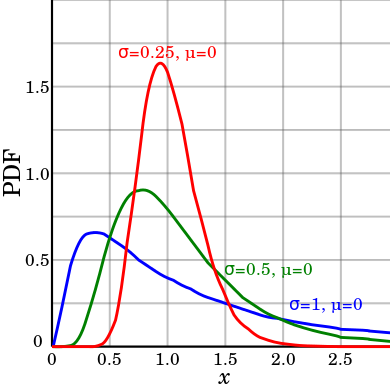
\includegraphics[width=1.5in]{./images/log-normal-dist.png}  \hfill \\
 
\subsubsection{Pareto distribution} 
Named after the economist Vilfredo Pareto, who used it to describe the distribution of wealth. \hfill \\
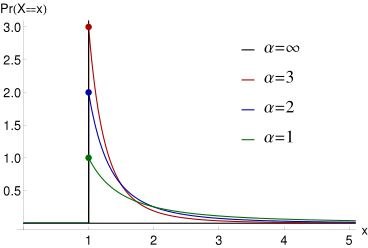
\includegraphics[width=1.5in]{./images/pareto-dist.png}  \hfill \\
Pareto distributions are often the result of generative processes with positive feedback

\subsection{Kernel density estimation}
A way to estimate the probability density function (PDF) of a random variable from a sample, in a non-parametric way.
\href{https://docs.scipy.org/doc/scipy/reference/generated/scipy.stats.gaussian_kde.html}{Scipy} has an implementation that automatically selects the kernel bandwidth. 
You can then get a non-parametric PDF, or use the method that samples from it. 

\subsection{Correlation}

\subsubsection{Pearson correlation}
$\displaystyle \rho = \frac{Cov(X,Y)}{S_X S_Y}$
Nicer to report than covariances, because its dimensionless, and the range is [-1, 1].
Works well if the relationship between variables is linear and if the variables are roughly normal.

\subsubsection{Spearman�s rank correlation}
Want more robustness in the presence of outliers?  Try Spearman's rank correlation.
To compute: compute the rank of each value, then compute Pearson�s correlation for the ranks. 
Can give higher correlations when the relationship is nonlinear or the distributions are skewed.  

\section{Biased \& unbiased estimators}
Variance is a biased estimator: when you have a sample that is small, you will under-estimate the variance of the underlying distribution. 
Amazingly, an unbiased estimator for variance: $s^2 = \frac{1}{n} (x_i - \bar{x})^2$ is  $s^2 = \frac{1}{(n - 1)} (x_i - \bar{x})^2$ 
The sample mean is unbiased. 

\section{Summarizing sample distributions}

Always keep in mind that the sampling distribution does not account for other sources of error, 
	notably sampling bias and measurement error.

After you parameterize a distribution, how do you report it? 
\begin{itemize}
	\item \textbf{Standard error} (SE) = $\sigma/\sqrt{n}$ is a measure of how far we expect the estimate to be off, on average. 
		For each simulated experiment, we compute the error, $\bar{x} ? ?$, 
			and then compute the root mean squared error (RMSE). 
		Note: as sample size increases, standard error gets smaller; standard deviation does not.
	\item \textbf{Confidence interval} (CI): a range that includes a given fraction of the sampling distribution. 
\end{itemize}
	
\subsubsection{SD vs SE}
\begin{itemize}
	\item The SD (standard deviation) quantifies scatter � how much the values vary from one another.
	\item The SEM (standard error of the mean) quantifies how precisely you know the true mean of the population. 
		It takes into account both the value of the SD and the sample size.
	\item Both SD and SEM are in the same units -- the units of the data.
	\item The SEM, by definition, is always smaller than the SD.
	\item The SEM gets smaller as your samples get larger. 
	\item The SD does not change predictably as you acquire more data. 
\end{itemize}

People often think that there is a 90\% probability that the actual parameter, $\mu$, falls in the 90\% confidence interval. 
Sadly, that is not true. 
If you want to make a claim like that, you have to use Bayesian methods
